\chapter{Elementos de la teoría musical}
\label{chap1}

El estudio de disciplinas como la música y las matemáticas requieren de una sólida comprensión de diversos conceptos esenciales. En este capítulo se introducen ideas básicas de la teoría musical, su terminología desde una visión amplia y genérica y la relación que guardan con conceptos físicos y matemáticos fundamentales. Estas nociones previas sientan las bases para comprender los algoritmos, aplicaciones y métodos que se explican en capítulos posteriores.

\section{Ondas y sonido}

\subsection{Ecuación de onda}

El \textbf{sonido} es una impresión producida en el oído causada por las vibraciones elásticas de un cuerpo que se propagan por el aire (u otros medios materiales) en forma de ondas. Muy a menudo, sin embargo, también nos referimos a él como la forma de energía que produce esta sensación. Mientras que la primera concepción, más sensorial, se relaciona con una perspectiva más artística, la segunda, más física, es la que tomamos cuando queremos hacer un análisis más objetivo de este fenómeno.

Para describir ondas y vibraciones, en matemáticas, se utilizan funciones trigonométricas. Los sonidos que se transmiten en forma de onda simple se denominan \textit{tonos puros} y se representan como:

%%% ACÍ hi ha PROBLEMES TAMBÉ
\begin{center}
\begin{minipage}[c]{0.45\textwidth} % Minipage per a l'equació i el text de descripció
    \vspace*{\fill} % Centra verticalment el contingut
    \begin{equation} 
        \label{eq.onda}
        u(t) = A \sin(2\pi \omega t-\phi)     
    \end{equation}
    
    \vspace*{\fill}
\end{minipage}
\begin{minipage}[c]{0.5\textwidth} 
    \centering
    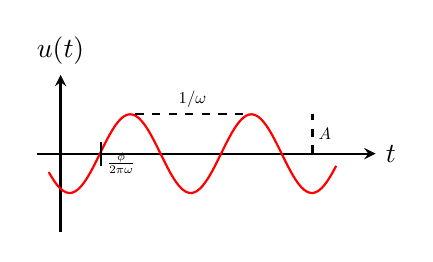
\begin{tikzpicture}[>=stealth, thick]
        \draw[->] (-0.8,0) -- (3.5,0) node[right] {$t$};
        \draw[->] (-0.5,-1) -- (-0.5,1) node[above] {$u(t)$};
        
        % Sinusoide
        \draw[red, thick, domain=-0.65:3.0, samples=100] 
            plot (\x, {0.5*sin(0.65*2*pi*\x r)});
        \draw[dashed] (2.7,0) -- (2.7,0.5) node[midway, right, scale=0.6] {$A$};
        \draw[dashed] (0.45,0.5) -- (1.9,0.5) node[above, midway, scale=0.6] {$1/\omega$};
        \draw[black, thick, shorten >=-1.5pt, shorten <=-1.5pt]  (0.015,-0.1) -- (0.015,0.1) node[below, anchor= north west, scale=0.6]{$\frac{\phi}{2\pi \omega}$};
    \end{tikzpicture}
\end{minipage}
\end{center}
Un tono es la percepción que se tiene de la frecuencia de un sonido. En la Música actual se eligen
algunos tonos fijos para realizar y escribir las composiciones, como es el caso de los que conforman la
escala cromática equitemperada que se verá posteriormente. En el apartado de características del sonido lo veremos como la \textit{altura}.

En la expresión de función de onda $u(t)$ aparecen los siguientes parámetros:
\begin{itemize}
    \item $t:$ representa el tiempo.
    \item \textbf{Amplitud de la onda}, $(A)$: magnitud máxima de desplazamiento de las partículas del medio desde su posición de equilibrio cuando una onda sonora pasa a través de ellas. Está directamente relacionada con la energía de la onda y, por lo tanto, con la intensidad acústica y la sonoridad percibida del sonido. Una mayor amplitud significa un sonido más intenso.
    \item \textbf{Fase}, $(\phi)$: describe la posición de una onda en un instante específico de tiempo. Indica el punto de su ciclo en el que comienza la onda. Aunque no afecta directamente a la altura o la sonoridad de un sonido individual, es crucial cuando se combinan múltiples ondas, ya que puede influir en la forma de la onda resultante y en fenómenos como la interferencia.
    \item \textbf{Frecuencia}, $(\omega)$: número de ciclos completos que una onda realiza en una unidad de tiempo. Se mide en \textit{Herzios} (Hz), donde $1 $ Hz equivale a un ciclo por segundo. Una mayor frecuencia corresponde a un sonido más agudo, mientras que una menor frecuencia se asocia con un sonido más grave.
\end{itemize} 
%%Características del sonido

\subsection{Características del sonido}
A partir de estos conceptos se pueden introducir algunas de las principales características del sonido desde un punto de vista más sensorial para el ser humano:
\begin{itemize}

\item \textit{\textbf{Altura:}} también conocido como \textit{tono} en castellano, es la cualidad del sonido que nos permite distinguir uno de otro y ordenarlos en una escala que va desde los más graves hasta los más agudos. No todos los sonidos tienen una altura definida. Sin embargo, en el caso de sonidos simples, la altura se corresponde directamente con su \textit{frecuencia}. Para las notas musicales producidas por un instrumento, la altura se asocia con la frecuencia más baja de todas las que componen el sonido (como veremos más adelante).

\item \textit{\textbf{Intensidad acústica:}} magnitud física (objetiva) que mide la potencia del sonido por unidad de área, expresada en \textit{watios} por metro cuadrado ($W/m^2$). Depende directamente de la \textit{amplitud de onda}: a mayor amplitud, mayor energía transporta la onda y, por lo tanto, mayor intensidad. Además, es la medida física que subyace a la percepción de la sonoridad. También se define como la cantidad de energía acústica que contiene un sonido. El nivel de intensidad, $\beta$, se mide en decibelios ($d\beta$) y se define como:
\begin{center}
\begin{minipage}[c]{0.45\textwidth}
\[
\beta=\log\frac{I}{I_0}
\]    
\end{minipage}
\begin{minipage}[c]{0.45\textwidth}
\begin{itemize}
    \item $I\equiv$ intensidad del sonido
    \item $I_0\equiv$ intensidad umbral de audición ($10^{-12}\ W/m^2$)
\end{itemize}
   
\end{minipage}

    
\end{center}

\item \textit{\textbf{Sonoridad:}} grado de sensación sonora (subjetiva) producida por un sonido de una determinada intensidad acústica. Para tonos puros, la sonoridad está directamente relacionada con la \textit{amplitud de onda}. De una manera menos precisa, a menudo se le denomina volumen.

\item \textit{\textbf{Timbre:}} cualidad del sonido que nos permite distinguir dos sonidos que tienen la misma altura y sonoridad. Depende directamente del \textit{espectro} del sonido (cantidad e intensidad de armónicos que lo componen). El timbre es lo que nos permite diferenciar, por ejemplo, una flauta de un violín tocando la misma nota a la misma intensidad.

\end{itemize}

\subsection{Serie harmónica}

Si bien se ha indicado que los tonos puros se transmiten como una onda sinusoidal simple descrita por (\ref{eq.onda}), en el mundo real, los sonidos que percibimos y que forman la base de la música son sonidos complejos. Los sonidos complejos se corresponden, matemáticamente, con combinaciones lineales de tonos puros. En otras palabras, cualquier sonido periódico puede ser visto como la superposición de múltiples ondas sinusoidales de diferentes amplitudes, frecuencias y fases.
%%Análisis de Fourier

La razón por la que en el análisis de un sonido musical solo aparecen múltiplos enteros de una frecuencia base no es una mera abstracción matemática, sino un reflejo directo de la física de los instrumentos. Consideremos el ejemplo más intuitivo: una cuerda de guitarra.

\begin{figure}[h!]
    \centering
    \includegraphics[width=0.55\linewidth]{Plantilla-LaTeX-TFG/images/harmonic_serie.png}
    \caption{Serie harmónica de \textit{la}$_2$. \texttt{/Users/dariosango44/Downloads/TFG Mates/python_tfg/harmonic_series_ii.py}}
    \label{fig:harmonic_serie}
\end{figure}

Cuando se pulsa, la cuerda vibra en toda su longitud, produciendo su frecuencia más grave, la \textit{frecuencia fundamental} ($f_1$). Esta es la nota que percibimos como el tono principal. Sin embargo, la cuerda no vibra únicamente de esta forma. Simultáneamente, y con menor amplitud, vibra en secciones más pequeñas, creando nodos (puntos que no se mueven) a lo largo de su longitud:
\begin{itemize}
    \item Vibra dividida en \textbf{dos mitades}, produciendo una frecuencia $f_2 = 2 \cdot f_1$. Este es el segundo armónico, que suena una octava por encima de la fundamental.
    \item Vibra dividida en \textbf{tres tercios}, produciendo una frecuencia $f_3 = 3 \cdot f_1$. Este es el tercer armónico, que suena una octava y una quinta por encima.
    \item En general, para cualquier entero $n \ge 1$, la cuerda puede vibrar en $n$ segmentos, produciendo el $n$-ésimo armónico con una frecuencia de $f_n = n \cdot f_1$.
\end{itemize}

El conjunto de todas estas frecuencias $\{f_1, 2f_1, 3f_1, \dots\}$ se conoce como la \textit{\textbf{serie armónica}} del sonido. La \textit{amplitud} de cada uno de estos armónicos es lo que define el \textit{timbre} de un instrumento, que como ya se ha indicado,  permite distinguir entre un violín y una flauta aunque ambos toquen la misma nota (la misma frecuencia fundamental).

La capacidad de analizar y descomponer un sonido complejo en sus distintas componentes de frecuencia (es decir, en una suma de tonos puros) es la piedra angular del Análisis de Fourier. Esta poderosa herramienta matemática es, entre otras, fundamental para la acústica y la teoría musical, ya que permite transformar una señal en el dominio del tiempo (cómo la amplitud varía con el tiempo) a una representación en el dominio de la frecuencia (qué frecuencias están presentes y con qué intensidad). Esto es posible gracias al siguiente resultado clave:

\begin{theorem}[De Fourier para señales periódicas]
Cualquier función periódica $f(t)$ de periodo $T$, (frecuencia fundamental $\omega=1/T$), se puede escribir como la suma numerable de funciones sinusoidales con frecuencias múltiplos enteros de $\omega$:
\[
f(t) \approx a_0+\sum_{n=1}^{\infty}(a_n\cos(n\omega t)+b_n\sin(n\omega t))
\]
donde los coeficientes de Fourier se calculan como: 
\begin{align*}
    a_0 &= \frac{1}{T} \int_0^T f(t) dt \\
    a_n &= \frac{2}{T} \int_0^T f(t) \cos(n\omega t) dt, \quad \text{para } n \ge 1 \\
    b_n &= \frac{2}{T} \int_0^T f(t) \sin(n\omega t) dt, \quad \text{para } n \ge 1
\end{align*}
\end{theorem}

\begin{figure}[h!]

\begin{minipage}{0.45\textwidth}
    \raggedright  
    \includegraphics[width=7cm]{Plantilla-LaTeX-TFG/images/pure_waves.png}
    \vspace{-0.8cm}
    \caption{Ondas puras.}\label{wave_pure}
\end{minipage}
\hfill
\begin{minipage}{0.45\textwidth}
    \raggedleft  
    \includegraphics[width=7cm]{Plantilla-LaTeX-TFG/images/wave_complex.png}
    \vspace{-0.8cm}   
    \caption{Onda compleja.}\label{wave_complex}
\end{minipage}

\caption{\texttt{/Users/dariosango44/Downloads/TFG Mates/python_tfg/fourier.py}}
\end{figure}

A partir de este teorema, que no demostraré porque hacerlo se escapa de los objetivos de este proyecto, se deduce que un sonido musical cotidiano (que es una onda periódica en el tiempo, al menos en periodos cortos) no es una entidad indivisible, sino un entramado de ondas sinusoidales más simples. En concreto:
\begin{itemize}
    \item La frecuencia $\omega$ es la frecuencia fundamental del sonido, que es la que percibimos como la altura de la nota.
    \item Las frecuencias $\omega,2\omega,...,n\omega$ son las frecuencias  de los sucesivos armónicos.
    \item Los coeficientes $a_n$ y $b_n$ determinan la amplitud relativa de cada armónico y la combinación específica de estas amplitudes es lo que le da a cada instrumento su timbre único, permitiéndonos distinguir una flauta de un violín, incluso si tocan la misma nota a la misma intensidad.

\end{itemize}
%\begin{remark}
 %   En la sección 1.2. se introduce el concepto de armónico.
%\end{remark}    
Este resultado es de vital importancia, ya que nos proporciona un marco matemático para entender la composición de los sonidos musicales y, por extensión, para la síntesis de sonido, el análisis de instrumentos y la teoría de la armonía.


\section{Sistema temperado y armonía}

%%%\subsubsection{Sistema y notación}
El espectro sonoro que el ser humano es capaz de percibir es continuo. En comparación con otras especies, los humanos tenemos un rango audible más limitado que no nos permite captar ultrasonidos (frecuencias superiores a 20.000 Hz), a diferencia de animales como los perros o los murciélagos. Lo mismo ocurre con los infrasonidos (frecuencias inferiores a 20 Hz), que el oído no percibe pero sí pueden sentirse como vibraciones en el cuerpo. \\

Para poder estudiar y organizar este espectro continuo, la evolución ha llevado a que la música occidental lo discretice en segmentos llamados \textit{notas}. La división empleada establece una repetición cíclica cada 12 notas, \(\mathbb{Z_{\text{12}}}\), de modo que al alcanzar la duodécima se retorna a la nota de partida, pero en una nueva octava (es decir, con el doble o la mitad de frecuencia). En este sistema la distancia entre dos notas consecutivas cualesquiera es de un \textit{semitono} ($\tfrac{1}{2}$ tono), la unidad mínima de intervalo en el sistema temperado occidental.\\

Cabe aclarar que en esta sección se presenta únicamente una descripción general del sistema de división del espectro audible. Los aspectos más detallados sobre el \textit{sistema temperado}, su origen histórico a partir de la afinación pitagórica y sus implicaciones en la afinación moderna serán desarrollados en el capítulo \ref{chap4}.\\

Las 12 notas del sistema temperado occidental, que conforman la conocida como \textbf{\textit{escala cromática}}, son las siguientes:
\begin{table}[h!]
    \centering
    \label{tab:notas_numeros}
    \begin{tabular}{cccccccccccl}
        \toprule
        \texttt{\textbf{do}} & \texttt{\textbf{do}}$\sharp$ & \texttt{\textbf{re}} & \texttt{\textbf{mi}}$\flat$ & \texttt{\textbf{mi}} & \texttt{\textbf{fa}} & \texttt{\textbf{fa}}$\sharp$ & \texttt{\textbf{sol}} & \texttt{\textbf{sol}}$\sharp$ & \texttt{\textbf{la}} & \texttt{\textbf{si}}$\flat$ & \texttt{\textbf{si}} \\   
        \hline
        C & C$\sharp$ & D & E$\flat$ & E & F & F$\sharp$ & G & G$\sharp$ & A & B$\flat$ & B \\
        \hline
         0 & 1 & 2 & 3 & 4 & 5 & 6 & 7 & 8 & 9 & 10 & 11 \\
        \bottomrule
    \end{tabular}
\end{table}\\

Las dos primeras filas muestran la correspondencia entre la notación latina y el cifrado americano y los símbolos $\sharp$ y $\flat$ representan, respectivamente, el \textit{sostenido} y el \textit{bemol}, que indican una alteración de la nota base a la que acompañan, incrementando o reduciendo su altura en un semitono. Por tanto, se deduce que notas como el Do$\sharp$ y el Re$\flat$ presentan el mismo sonido (en el sistema occidental de afinación), fenómeno recibe el nombre de \textit{enarmonía}.\\

\begin{figure}
    \centering
    \includegraphics[width=0.5\linewidth]{Plantilla-LaTeX-TFG/images/cromaticScale.png}
    \caption{Escala cromática del temperamento igual.}
    \label{fig:escala_cromatica}
\end{figure}

Para observar fácilmente los conceptos anteriores visualicemos el siguiente teclado de un piano:
\\
\begin{figure}[h!]
    \centering
    \includegraphics[width=0.5\linewidth]{Plantilla-LaTeX-TFG/images/teclado-corto-1024x292.png}
    \caption{Teclado de un piano.}
    \label{fig:piano_keys}
\end{figure}
La imagen \ref{fig:piano_keys} permite comprender de forma intuitiva la distribución de tonos y semitonos. Si observamos dos teclas blancas consecutivas, notaremos que no siempre están separadas por la misma distancia sonora: entre \texttt{\textbf{mi--fa}} y entre \texttt{\textbf{si--do}} no existe tecla negra intermedia, lo que indica que esos pares de notas están separados únicamente por un \textit{semitono}. En los demás casos (por ejemplo, \texttt{\textbf{do--re}} o \texttt{\textbf{fa--sol}}), la presencia de una tecla negra entre ambas señala que la distancia es de un \textit{tono} completo, es decir, dos semitonos.
Esta alternancia de tonos y semitonos es la base sobre la cual se construyen las escalas del sistema occidental.\\
Además, haciendo sonar sucesivamente todas las teclas presentes -blancas y negras- entre el primer \texttt{\textbf{do}} y el inmediatamente superior tendríamos una representación de la anteriormente mencionada \textit{escala cromática} de 12 sonidos y si únicamente hiciéramos sonar las teclas blancas del mismo rango tendríamos una representación de la \textit{escala diatónica}, en este caso de \textit{Do Mayor}. Lo veremos con mayor detalle en la sección \ref{intro_scales}.


% En particular, la \textbf{escala mayor} sigue la siguiente secuencia de % % distancias:
% \[
% \text{Tono -- Tono -- Semitono -- Tono -- Tono -- Tono -- Semitono}.
% \]
% Aplicada a la nota Do como punto de partida, se obtiene la \textbf{escala de Do mayor}:
% \[
% \text{Do -- Re -- Mi -- Fa -- Sol -- La -- Si -- Do}.
% \]
% Cada octava repite este patrón, manteniendo las mismas relaciones de intervalo pero en diferentes registros.

%%%\subsubsection{Intervalos y Acordes}
\subsection{Intervalos}
La distancia entre notas musicales diferentes se puede medir de varias formas, cada una ofreciendo una perspectiva complementaria sobre la estructura musical. Desde un punto de vista cromático, basándose en las doce notas del sistema temperado occidental, la distancia se cuantifica en \textit{semitonos}. Por ejemplo, la distancia entre \texttt{\textbf{do}} y \texttt{\textbf{mi}} es de 4 semitonos. Visualizando diatónicamente, es decir, extendiendo la escala cromática, los intervalos se pueden identificar con el ordinal que expresa el número de notas que hay entre las que se calcula el intervalo, con estas incluidas, \textit{i.e.}, entre \texttt{\textbf{do}} y \texttt{\textbf{mi}} se tienen \texttt{\textbf{do}}, \texttt{\textbf{re}}, \texttt{\textbf{mi}}, por tanto se corresponde con una \textit{tercera mayor}. En lo referente al adjetivo que acompaña al ordinal, viene determinado por otras cualidades sonoras del intervalo y puede ser \textit{disminuido}, \textit{menor}, \textit{justo}, \textit{mayor} y \textit{aumentado}.

\begin{figure}[h!]
    \centering
    \includegraphics[width=0.5\linewidth]{Plantilla-LaTeX-TFG/images/intervals.png}
    \caption{Ejemplo de intervalos en Re Mayor.}
    \label{fig:intervals}
\end{figure}

Además de estas medidas, un intervalo también puede cuantificarse como la razón entre las frecuencias de los dos sonidos que lo componen. Por ejemplo, si consideramos las frecuencias aproximadas de \texttt{\textbf{do}} y \texttt{\textbf{mi}} en la octava central del piano (afinación por \textbf{temperamento igual}):
\[
\text{Int(\texttt{\textbf{do,mi}})}=\frac{f(\texttt{\textbf{mi}})}{f(\texttt{\textbf{do}})}\approx\frac{329.6275 Hz}{261.6265 Hz}\approx 1.25999
\]
El valor obtenido es la razón de frecuencias de una tercera mayor en el temperamento igual, que matemáticamente se define como $2^{4/12}=2^{1/3}$. Sin embargo, históricamente, los intervalos de consonancia perfecta se han definido por razones de enteros simples, que provienen de la serie armónica natural establecida por Pitágoras tras estudiar las propiedades de los sonidos producidos por el \textit{monocordio}, \textit{el yunque}...\\
Por tanto se puede establecer que, en general, dadas dos notas de frecuencias fundamentales $f_1$ y $f_2$ con $f_1>f_2$, el intervalo que forman lo podemos expresar como la razón $r=f_1/f_2$. Además, dado que esta escala es multiplicativa, para ``sumar'' dos intervalos multiplicaremos las
razones y para ``restarlos'' las dividiremos. Veamos:\\
\begin{example}
\label{calcul_interval}
    Dadas las razones interválicas justas de \texttt{\textbf{do-mi}}, $5/4$; y \texttt{\textbf{do-sol}}, $3/2$, calcular el intervalo \texttt{\textbf{mi-sol}}.
\end{example}
Con abuso de notación:
\[
\frac{\texttt{\textbf{sol}}}{\texttt{\textbf{do}}}=\frac{\texttt{\textbf{sol}}}{\texttt{\textbf{mi}}}\times\frac{\texttt{\textbf{mi}}}{\texttt{\textbf{do}}}
\]

Sustituyendo valores conocidos:
\[
\frac{3}{2}=r\times\frac{5}{4}
\]

Despejando:
\[
r=\frac{3/2}{5/4}=\frac{12}{10}=\frac{6}{5}
\]

La razón $6/5$ representa el intervalo que va de \texttt{\textbf{mi}} a \texttt{\textbf{sol}} en ese contexto de entonación pitagórica.
\begin{remark}
    En el capítulo \ref{chap4} se tratará en profundidad la evolución del sistema temperado y las afinaciones, que permiten entender mejor este ejemplo.
\end{remark}
De esta manera podemos ver que es posible establecer una relación entre los intervalos expresados en forma ordinal y la razón ideal entre frecuencias, como se muestra en la tabla siguiente, que presenta las fracciones para los intervalos pitagóricos principales:\\
\begin{table}[h!]
    \centering
    \begin{tabular}{|c|c|c|c|c|c|c|c|}
        \hline
         \texttt{do}&\texttt{re}&\texttt{mi}&\texttt{fa}&\texttt{sol}&\texttt{la}&\texttt{si}&\texttt{do}'  \\
         \hline
         -&2ª&3ª&4ª&5ª&6ª&7ª&8ª \\
         \hline
         1&9/8&5/4&81/64&3/2&27/16&243/128&2/1 \\
         \hline
    \end{tabular}
    \caption{Relación interválica pitagórica.}
    \label{tab:intervals_table}
    
\end{table}\\
Estas proporciones reflejan la relación matemática entre las notas dentro de una escala diatónica en afinación justa. Cabe destacar que en el sistema temperado igual, estas razones se aproximan ligeramente para permitir la modulación libre entre tonalidades, a costa de una leve desviación respecto a las proporciones puras.

\subsection{Acordes}
\label{section_chords}
Una vez se conoce el funcionamiento de los intervalos, el siguiente paso lógico se correponde con el concepto de \textbf{\textit{acorde}}. Cuando suenan simultáneamente tres o más notas diferentes se produce una combinación de sonidos denominada acorde. Los acordes se clasifican en función de los intervalos que presentan las notas que los separan. 

En la práctica musical, los acordes constituyen la base sobre la que se construye la armonía. Un acorde sencillo, llamado \textit{tríada}, se compone de tres notas: la \textit{fundamental}, la \textit{tercera} y la \textit{quinta}. La forma en que se organizan estas notas determina el tipo de acorde y su carácter sonoro.

Cada tipo de acorde tiene una sonoridad característica: el \textit{mayor} suele percibirse como estable o brillante, el \textit{menor} como más oscuro o melancólico, mientras que los \textit{aumentados} y \textit{disminuidos} generan tensión y se utilizan con frecuencia para crear movimiento o cambio armónico.

\begin{figure}[h!]
    \centering
    \includegraphics[width=0.5\linewidth]{Plantilla-LaTeX-TFG/images/american_chords.png}
    \caption{Acordes en notación americana.}
    \label{fig:chords}
\end{figure}

A partir de las tríadas se pueden formar acordes más complejos añadiendo nuevas notas, como la séptima, la \textit{novena} o la \textit{oncena}. Estos \textit{acordes extendidos} enriquecen la textura armónica y amplían las posibilidades expresivas de la música tonal.

En conjunto, los acordes constituyen la base tonal de la música occidental: son el marco en el que se desarrollan las melodías, las progresiones y, en definitiva, la sensación de tensión y resolución que caracteriza al lenguaje armónico.


\subsection{Armonía}
Para concluir la sección es necesario introducir el concepto que subyace a todo lo anteriormente expuesto y que ya ha aparecido en diferentes ocasiones a lo largo de la redacción: la armonía. 

Desde una perspectiva general y filosófica, la armonía se concibe como un concepto metafísico y se define como el equilibrio y la adecuada proporción entre las distintas partes de un todo, generando una sensación de cohesión y belleza. 

Musicalmente, la armonía puede definirse como el estudio de la relación entre sonidos que suenan simultáneamente (acordes) y cómo estos progresan a lo largo del tiempo. No se trata únicamente del ''equilibrio de proporciones'', sino también de cómo esas proporciones -los intervalos- crean sensaciones de tensión, reposo, consonancia y disonancia. 

En esencia, la armonía actúa como la ``columna vertebral'' del lenguaje tonal: los acordes definen el marco estructural, los intervalos establecen la calidad sonora, y las progresiones armónicas organizan la movilidad y el desarrollo en el tiempo. Esta comprensión de la armonía permitirá adentrarse en los siguientes capítulos, donde se abordarán con mayor profundidad todos estos aspectos.


\section{Escalas}
\label{intro_scales}
Una escala es un conjunto finito de notas ordenadas según su frecuencia fundamental. En el contexto de la música occidental, el inicio y el final de una escala cualquiera viene dado por las notas de frecuencias $f$ y $2f$, es decir, la nota fundamental y su correspondiente \textit{octava}. Si establecemos $\mathbb{R}^+:=(0,+\infty)$ como el conjunto de las frecuencias de las notas, matemáticamente, una escala se puede concebir de la siguiente manera: 
\begin{definition}[Escala]
   Es un subconjunto $E \subset \mathbb{R}^+$ tal que cumple las siguientes propiedades:
   \begin{enumerate}
       \item Existe una biyección $f:\mathbb{Z}\xrightarrow{}E$ que conserva el orden, \textit{i.e.}, si $i<j$, $f(i)<f(j)$ $\forall i,j \in \mathbb{Z}$.
       \item Si $u \in E$, entonces $2u$ y $u/2$ también pertenecen a $E$.
   \end{enumerate}
   De la propiedad (1) se deduce que una escala es ilimitada tanto superior como inferiormente y de la (2) se induce que si una escala contiene una nota, también contindrá la 8ª superior y la inferior.
\end{definition}
\begin{remark}
    Esta definición de escala se aclarará más adelante.
\end{remark}
\begin{example}[Escala mayor]
Una escala mayor consta de 7 notas cuyos intervalos sucesivos son todos \textit{segundas mayores} salvo entre la 2ª y la 3ª y la 7ª y la 1ª, que hay una distancia de semitono. Se tiene la sucesión de tonos: \(\{1,1,\frac{1}{2},1,1,1,\frac{1}{2}\}\).
    \begin{figure}[h!]
        \centering
        \includegraphics[width=0.25\linewidth]{Plantilla-LaTeX-TFG/images/FaM.png}
        \caption{Escala de Fa Mayor.}
        \label{fig:FaM}
    \end{figure}
\end{example}
\begin{example}[Escala de \textit{blues}]
La escala de \textit{blues} expuesta presenta seis notas derivada de la escala pentatónica menor, pero con una nota adicional llamada ''blue note''. Dicha nota añadida se corresponde con la \textit{quinta disminuida}, que le transfiere el característico sonido sucio y expresivo que caracteriza al género. En semitonos: \(\).
\begin{figure}[!h]
    \centering
    \includegraphics[width=0.45\linewidth]{Plantilla-LaTeX-TFG/images/hexatonic_blues_scale.png}
    \caption{Escala de hexatónica de \textit{blues}.}
    \label{fig:hexatonic_blues_scale}
\end{figure}
\end{example}
\begin{example}[Escala árabe o modo armónico.]
El modo armónico de la escala de Mi menor, también conocido como la escala árabe, se corresponde con la escala menor de \texttt{\textbf{mi}}, relativo de Sol Mayor, que consta de 7 notas y con la última alterada un semitono hacia arriba. En semitonos: \(\).
    \begin{figure}[h!]
        \centering
        \includegraphics[width=0.5\linewidth]{Plantilla-LaTeX-TFG/images/mim_harmonic.png}
        \caption{Escala árabe de Mi.}
        \label{fig:mim_harmonic}
    \end{figure}
\end{example} 
A continuación, tomando como premisa el sistema pitagórico de afinación se expondrá una herramienta que permite comprender de forma esquemática las relaciones entre las tonalidades más comunes de la música occidental.\\
Tras la razón de enteros $2/1$ referente a la \textit{octava}, la razón de enteros más importante para los Pitagóricos era el \(3/2\), que se corresponde con el intervalo de \textit{quinta justa}, (\ref{tab:intervals_table}.) Los discípulos de Pitágoras se percataron de que, recorriendo en intervalos sucesivos de quintas ascendentes a partir del Do, eran capaces de obtener una espiral de quintas de la siguiente forma:
\[
\footnotesize{\texttt{\textbf{do}}\xrightarrow{}\texttt{\textbf{sol}}\xrightarrow{}\texttt{\textbf{Re}}\xrightarrow{}\texttt{\textbf{la}}\xrightarrow{}\texttt{\textbf{mi}}\xrightarrow{}\texttt{\textbf{si}}\xrightarrow{}\texttt{\textbf{fa}}\sharp \xrightarrow{}\texttt{\textbf{do}}\sharp\xrightarrow{}\texttt{\textbf{sol}}\sharp\xrightarrow{}\texttt{\textbf{re}}\sharp\xrightarrow{}\texttt{\textbf{la}}\sharp\xrightarrow{}\texttt{\textbf{mi}}\sharp\xrightarrow{}\texttt{\textbf{si}}\sharp}
\]
En el sistema igualemente temperado existe una \textit{enarmonía} entre \texttt{\textbf{do}} y \texttt{\textbf{si}}$\sharp$ y entre \texttt{\textbf{fa}} y \texttt{\textbf{mi}}$\sharp$. En consecuencia, iterando ascendentemente intervalos de quintas podemos recorrer las 12 notas de la escala cromática. Igualmente, realizando intervalos sucesivos de quintas descendentes se obtiene que: 
\[
\footnotesize{\texttt{\textbf{do}}\xrightarrow{}\texttt{\textbf{fa}}\xrightarrow{}\texttt{\textbf{si}}\flat\xrightarrow{}\texttt{\textbf{mi}}\flat\xrightarrow{}\texttt{\textbf{la}}\flat\xrightarrow{}\texttt{\textbf{re}}\flat\xrightarrow{}\texttt{\textbf{sol}}\flat \xrightarrow{}\texttt{\textbf{do}}\flat\xrightarrow{}\texttt{\textbf{fa}}\flat\xrightarrow{}\texttt{\textbf{si}}\flat\flat\xrightarrow{}\texttt{\textbf{mi}}\flat\flat\xrightarrow{}\texttt{\textbf{la}}\flat\flat\xrightarrow{}\texttt{\textbf{re}}\flat\flat}
\]
Estas sucesiones de intervalos se transforman en cíclicas en ambas direcciones en el sentido en que, tras pasar por todas las notas de la escala cromática, vuelven al \texttt{\textbf{do}} original enarmonía mediante. Es importante recalcar que esto ocurre, como ya he dicho, en el sistema igualmente temperado, dado que el intervalo de quinta justa abarca exactamente 7 semitonos, no así en sistemas de afinación diferentes del igualmente temperado.\\ 
Pensando en teoría de números, lo que se está haciendo al desplazarse una quinta justa ascendente o descendentemente se corresponde con la operación de sumar $7\pmod{12}$. El denominado \textit{círculo de quintas} se genera al aplicar iterativamente:
\[
C_n=(C_{n-1} + 7) \pmod{12}, \quad n \in \mathbb{Z}_{12}
\]
El hecho de que 7 sea coprimo con 12, \textit{i.e.} mcd$(12,7)=1$, implica que 7 es un generador del grupo \(\mathbb{Z}_{12}\) y que tras aplicar la operación ''+'' doce veces, se recorren todas las clases del tono -notas- antes de regresar al punto de partida.
\[
7 \times 1 = 7 \pmod{12} \quad (\texttt{\textbf{sol}}) \\\]
\[7 \times 2 = 14 \equiv 2 \pmod{12} \quad (\texttt{\textbf{re}}) \\
\]
\[\dots\]
\[
7 \times 12 = 84 \equiv 0 \pmod{12} \quad (\texttt{\textbf{do}})
\]
Por ello, se puede construir el \textit{círculo de quintas}, que es la herramienta que se mencionaba anteriormente: \\
\begin{figure}[h!]
    \centering
    \includegraphics[width=0.45\linewidth]{Plantilla-LaTeX-TFG/images/fifth_circle.png}
    \caption{Espiral de quintas en cifrado americano que pone de relieve las diferencias entre notas propias de sistemas no igualemente temperados.}
    \label{fig:fifth_circle}
\end{figure}
Este diagrama actúa como un mapa que permite, según la interpretación que se le dé, acceder a diferente información íntimamente relacionada con las escalas y las tonalidades, y facilita el transporte de piezas musicales para poder ser interpretadas y leídas por diferentes instrumentos.\\

Para concluir y tras haber definido el concepto de escala, resulta natural introducir el concepto de tonalidad o en inglés, \textit{key}, que constituye el marco en el que funciona gran parte de la música occidental. La tonalidad se entiende como un sistema de organización musical en el cual una determinada nota, llamada \textit{tónica}, adquiere la máxima estabilidad, mientras que las demás notas y acordes se definen en relación con esta, que actúa como sistema de referencia.
Siguiendo esta perspectiva, podemos decir que una obra o fragmento es tonal cuando:
\begin{itemize}
  \item Existe una nota (la tónica) que actúa como “hogar” sonoro, hacia la cual las melodías y progresiones armónicas tienden a regresar.  
  \item La escala utilizada (o las notas predominantes) pertenecen a un conjunto coherente (por ejemplo la escala mayor o menor) que refuerza esa tónica.   
\end{itemize}
\begin{figure}
    \centering
    \includegraphics[width=0.5\linewidth]{Plantilla-LaTeX-TFG/images/Circle_of_fifths.png}
    \caption{Círculo de quintas con tonalidades.}
    \label{fig:Circle_of_fifths}
\end{figure}
La figura \ref{fig:Circle_of_fifths} puede interpretarse como una representación gráfica y modular de estas relaciones tonales. Cada posición en el círculo corresponde a una tonalidad mayor (y su relativa menor), y los desplazamientos entre posiciones adyacentes reflejan una cercanía tonal determinada por el número de notas comunes entre escalas. Dos tonalidades vecinas en el círculo —por ejemplo, Do Mayor y Sol Mayor— difieren únicamente en una alteración (un sostenido o un bemol), lo que las hace armónicamente compatibles y facilita las modulaciones suaves entre ellas.\\
A medida que se avanza en el círculo hacia tonalidades más alejadas, el número de alteraciones aumenta y la relación interválica con la tónica inicial se debilita. En consecuencia, tonalidades opuestas en el círculo —como Do Mayor y Fa$\sharp$ Mayor— presentan máxima lejanía tonal, compartiendo pocas notas y generando un contraste más intenso en el discurso musical.\\
Además, el círculo de quintas permite visualizar de forma directa las relaciones entre tonalidades relativas (una mayor y su menor comparten la misma armadura de clave) y las relaciones de dominante y subdominante (quintas ascendentes y descendentes respecto a la tónica).\\

En definitiva, el círculo de quintas constituye una herramienta que integra en un solo esquema la teoría de intervalos, la estructura de las escalas y la organización de las tonalidades. Permite comprender cómo la afinación basada en razones simples (como 3/2 o 2/1) da lugar a un sistema cerrado de doce sonidos interrelacionados, dentro del cual emergen las nociones de cercanía tonal, modulación y jerarquía funcional. Su interpretación, tanto desde el punto de vista matemático como musical, revela la profunda conexión entre proporción, simetría y percepción sonora que caracteriza la música occidental.

\section{Ritmo}
\label{rythm}

A diferencia de la altura musical, que se organiza en el dominio de las frecuencias, el ritmo opera sobre el dominio lineal del tiempo, el cual es dividido y agrupado. La formalización matemática de este dominio se basa en estructuras discretas, aritmética de fracciones y teoría de conjuntos para modelar las duraciones relativas y la periodicidad.\\
A continuación, se expondrán los elementos esenciales para la comprensión del tiempo musical, haciendo especial énfasis en cómo el ritmo y la métrica imponen una estructura jerárquica y proporcional sobre el eje temporal.\\

Para transcribir y analizar la música es necesario cuantificar la duración de los eventos sonoros (notas) y no sonoros (silencios). Esta cuantificación se realiza mediante la división sistemática del tiempo a través de elementos como:
\begin{itemize}
    \item \textit{\textbf{Pulso}}: es el elemento fundamental para la medición del ritmo, también conocido como \textit{beat}. Matemáticamente, el pulso se establece como una unidad de tiempo constante y fija $t\in \mathbb{R^+}$. Se corresponde con el ''\textit{latido}'' de los fragmentos musicales y se mide de igual manera, en \textit{pulsos por minuto.} En las partituras musicales, que son el medio material más común sobre el que se escribe la música, se acostumbra a escribir algo como:

    %% PROBLEMES ACÍ
    \[
        \musQuarter .  = 76
    \]

    
    que indica los pulsos por minuto que debe marcar un metrónomo.

    \item \textit{\textbf{Duración}}: se define como una medida relativa al pulso, siendo siempre un múltiplo racional de $t$, es decir:
    \[
    d=r\cdot t, \quad r \in \mathbb{Q}^+ 
    \]
    Además, como las duraciones posibles se encuentran en el conjunto \(\mathbb{Q^+}\) y son generalemente binarias o ternarias, se puede modelar un conjunto adaptado de duraciones $\mathcal{D}$ de la siguiente forma:
    \[
    \mathcal{D}=\{t\cdot \frac{m}{2^a3^b}: m,a,b \in \mathbb{N}\}
    \]
    \item \textit{\textbf{Compás}}: usualmente se expresa como una fracción al principio de las partituras, $\frac{N}{U}$, donde el numerador ($N$) expresa la longitud del ciclo en pulsos $t$ que caben en un compás y el denominador ($U$) define la figura rítmica que toma el valor de la unidad de pulso. 
    
\end{itemize}
\begin{example}
    En el fragmento la obra de Mozart (\ref{fig:Mozart_minuet}), el compás empleado es el $6/8$. El denominador $U=8$ indica que la corchea es la unidad de cuenta. El numerador $N=6$ indica seis de estas unidades por ciclo. Sin embargo, este compás es una métrica compuesta, agrupándose en solo dos pulsos principales con subdivisión ternaria. Así, la unidad de pulso efectivo $t$ es la negra con punto ($3/8$ de una redonda). El $6/8$ se comporta como un ciclo binario ($\mathbb{Z}_2$) en su nivel superior de acento, pero como un subciclo ternario ($\mathbb{Z}_6$) en su nivel de subdivisión.
    
        \begin{figure}[h!]
            \centering
            \includegraphics[width=0.5\linewidth]{Plantilla-LaTeX-TFG/images/MozartExcerptK331.svg.png}
            \caption{Extracto de obra de compás de subdivisión ternaria.}
            \label{fig:Mozart_minuet}
        \end{figure}
        
\end{example}
El sistema occidental de notación rítmica se basa históricamente en la división binaria, un principio de partición recursiva donde cada duración se divide generalmente en dos tiempos iguales. Este principio genera las figuras rítmicas principales (redonda, blanca, negra, corchea, semicorchea, etc.) a través de una progresión geométrica de razón 1/2 sobre la duración de referencia $t$, que suele ser la \textit{negra}.\\
%%% AQUÍ TABLA DE VAINAS BACANAS --  Duración notas %%%
\begin{table}[h!]
            \centering
            \label{tempos_figures}
            \begin{tabular}{|c|c|}
                \hline
                 \textbf{Figura}&\textbf{Tiempos}  \\
                 \hline
                 Redonda ($\musWhole$)&4\\
                 Blanca ($\musHalf$)&2\\
                 Negra ($\musQuarter$)&1 \\
                 Corchea ($\musEighth$)& 1/2\\
                 Semicorchea ($\musSixteenth$)&1/4 \\
                 \hline
            \end{tabular}
            \caption{Tiempos y figuras tomando a la \textit{negra }como referencia.}
            \label{tab:table_temps}
\end{table}

En conclusión, se puede percibir el compás como un ciclo temporal de orden $n$ y modelar el conjunto de pulsos dentro de un compás mediante el grupo cíclico 
\[
\mathbb{Z}_n=\{0,1,2,\ldots,n-1\}
\]
bajo la adición módulo $n$ y donde la posición de un pulso $p$ en el ciclo se identifica con su resto $\pmod n$.